\chapter{Implementierung}
\label{chap:Implementierung}

\section{Editor}
\label{sec:Editor}
Der Editor ist die Schnittstelle der DSL mit einem menschlichen Benutzer. Hier wird ein DSL-Modell durch Interaktion mit der konkreten Syntax erstellt oder bearbeitet. Die konkrete Syntax nimmt die Form eines Graphen an, der in Kapitel \ref{chap:Einleitung} beschrieben ist. Die Aufgabe des Editors ist es, die konkrete Syntax in abstrakte Syntax umzuwandeln. Während der Benutzer über die grafische Benutzeroberfläche mit der konkreten Syntax interagiert, also Instruktionen hinzufügt und Verbindungen zieht, wird Editor-intern die abstrakte Syntax geformt, welche der Benutzer nicht sieht (vgl. [CITATION Voelter, DSL Engineering, Abs 3.4, PDF Seite 68]. Die abstrakte Syntax ist durch eine C\#-Datenstruktur repräsentiert, welche für die weiteren Verarbeitungsschritte gespeichert wird (siehe Abschnitt \ref{sec:Verarbeitungsschritte}). In der Literatur wird die Datenstruktur, welche die abstrakte Syntax beinhaltet, auch semantisches Modell (engl. semantic model) genannt, vgl. [CITATION Martin Fowler, Domain Specific Languages] und wird daher im Folgenden auch so referenziert. Der Editor bildet also die abstrakte Syntax auf das semantische Modell ab. Diese Abbildung ist bidirektional: Wird das semantische Modell manipuliert, spiegelt die grafische Benutzeroberfläche dies in der konkreten Syntax wider.
\newline
Der Editor ist als eine Windows Forms-Anwendung umgesetzt und implementiert das Model-View-Viewmodel-Entwicklungsmuster (kurz MVVM). Ähnlich wie bei verwandten Entwurfsmustern wie zum Beispiel Model-View-Controller (MVC) geht es bei MVVM darum, die Darstellung einer Anwendung von ihrer Logik zu trennen. Dies geschieht durch eine Einteilung in drei verschiedene Schichten: Dem View, dem Viewmodel und dem Model. Die View-Schicht dient zur Darstellung der Anwendung und umfasst die Komponenten der grafischen Benutzeroberfläche. Sie erhält die nötigen Daten zur Darstellung vom Viewmodel über sogenannte Datenbindung (engl. Data Binding). Dabei werden Daten über ein Framework an einander gebunden und werden so vom System bei jeder Zustandsänderung synchron gehalten. Ändern sich also Daten im Viewmodel wird dies unverzüglich im View angezeigt. Das Viewmodel kümmert sich um die Präsentationslogik, das heißt es ist dafür zuständig, dem View Daten zur Verfügung zu stellen, welche über Datenbindungen angezeigt werden sollen. Dafür hat das Viewmodel Zugriff auf das Model, über dass die Daten zur Darstellung abgerufen werden. Im Model werden auch die Geschäftslogik sowie Speicher- und Lade-Aktionen ausgeführt. In .NET wird MVVM vor allem im Zuge der Windows Presentation Foundation eingesetzt, kann aber auch durch das Devexpress-Framework in Windows Forms-Anwendungen benutzt werden.
\newline
Im grafischen Editor der DSL werden die drei Schichten von MVVM durch verschiedene C\#-Klassen abgebildet, welche im Folgenden erläutert werden.

\subsection{Die Model-Schicht: Flow, Node, Input, Output, Connector, Variable, Function}
\label{subsec:Die Model-Schicht}
Die Model-Schicht beinhaltet die C\#-Datenstruktur, welche auch als semantisches Modell bezeichnet wird: Also das Objekt, welches in der weiteren Verarbeitung die abstrakte Syntax beschreibt. Das semantische Modell selbst weist kein programmitisches Verhalten auf, sondern ist eine reine Datenstruktur. Es besteht aus Instanzen von Klassen, welche die einzelnen Elemente der DSL modellieren und im Namespace ilogixx.ConversationFlow.Core definiert sind. Die Klassenstruktur der Model-Schicht ist in Abbildung [IMAGE UML MODEL] als UML-Diagramm aufgeführt und wird im Folgenden erläutert.
\newline
Instruktionen werden durch die abstrakte Klasse Node modelliert. Node besitzt eine Liste von Referenzen auf Output-Objekte, welche die Ausgänge einer Intruktion modellieren. Node hat ebenfalls eine Referenz auf ein Objekt vom Typ Input, welches den Eingang eines Knotens symbolisiert. Jede Art von Instruktion hat ihre eigene Subklasse, welche die Instruktionen aus Abschnitt \ref{sec:Sprachelemente} abbilden. Pro Ausgang einer Instruktion fügt der Konstruktor des Subtypen eine Referenz vom Typen Output der Referenzliste der Basisklasse hinzu. Im Konstruktor wird ebenfalls der Input spezifiziert: Hat die Instruktion einen Eingang, wird die Input-Referenz instanziert, andernfalls bleibt sie null. Viele Instruktionen haben die gleiche Anzahl an Ausgängen und einen Eingang. Daher existieren Subtypen, welche diese Initialisierungsarbeit übernehmen: Inputnode, für Instruktionen die einen Eingang haben, SingleOutputNode für Instruktionen die einen einzelnen Ausgang haben, und SingleThroughputNode, für Instruktionen die einen Ein- und einen einzelnen Ausgang haben. Alle elf Subtypen für die Instruktionen erben von diesen drei Klassen und passen dort wo nötig ihre Konfiguration an. Beispielsweise erbt DTMFCharacterNode von InputNode, und fügt der Output-Referenzliste dreizehn neue Outputs hinzu.
\newline
Die Klasse Input ist simpel: Sie zeigt über eine Referenz vom Typen Node auf ihre besitzende Instruktion. Die Klasse Output hingegen besitzt einige mehrere Daten. Sie speichert den Bezeichner des Ausgangs als String, einen weiteren String namens DisplayString, welcher vom Benutzer editiert werden kann und auf der Benutzeroberfläche angezeigt wird, einen Boolean namens Visible, welcher bestimmt ob der Ausgang in dem Rechteck der beinhaltenden Instruktion angezeigt wird, und eine Referenz vom Typ Input auf einen Eingang, falls der Ausgang mit einem solchen verbunden sein sollte. Durch letztere Input-Referenz sind die Verbindungen im Konversationsrouting zwischen den Instruktionen implizit gegeben. Dennoch existiert eine weitere Klasse namens Connector, welche eine Verbindung explizit definiert. Sie besitzt Referenzen auf die Input- und die Output-Instanz, welche verbunden sind.
\newline
Benutzerdefinierte Variablen und Funktionen sind über eigene Klassen abgebildet: Variable und Function. Variable besitzen einen Namen vom Typen String und einen Typen, der über einen Enum namens VariableType abgebildet ist, welcher die in \ref{subsec:Variablen} aufgezählten Typen beinhaltet. Function speichert ebenfalls einen Namen vom Typen String und einen Rückgabetyp, welcher über einen Enum mit Namen FunctionReturnType abgebildet ist. Zusätzlich wird der Funktionskörper mit Namen Body als String gespeichert. Parameter einer Funktion werden über eine Liste von Referenzen auf Objekte des Type Parameter modelliert. Ein Parameter besitzt, ähnlich wie die Klasse Variable, einen Namen als String und einen Typen als VariableType. Die Klasse Flow vereint alle oben genannten Klassen: Sie beinhaltet Listen mit Referenzen auf alle Nodes, Connectors, Functions und Variables. 

\subsection{Die Viewmodel-Schicht: FlowDiagramViewmodel, CodeEditorViewModel, FunctionCollectionEditorViewModel}
\label{subsec:Die Viewmodel-Schicht}
In der Viewmodel-Schicht werden die Klasseninstanzen der Model-Schicht so aufbereitet, dass die View-Schicht sie per Datenbindung repräsentieren kann. Die Viewmodel-Schicht reagiert auch auf Eingaben des Benutzers und manipuliert das zu Grunde liegende Model nach dessen Wünschen. 
\newline
Der Hauptbestandteil dieser Schicht ist die Klasse FlowDiagramViewmodel. Diese besitzt als Member-Variablen Listen auf Referenzen der Model-Komponenten Node, Connector, Variable und Function. Diese Listen sind vom .NET-Typ ObservableCollection, welche ein Event auslösen, falls der Liste Objekte hinzugefügt oder entfernt werden. Diese Listen sind per Devexpress-Datenbindung an die View-Schicht gekoppelt. Das heißt, wenn auf der View-Schicht Elemente des Models wie neue Node- oder Connector-Objekte hinzugefügt werden, aktualisieren sich die entsprechenden Listen im FlowDiagramViewmodel. Zusätzlich werden dadurch Events ausgelöst, auf die FlowDiagramViewModel reagiert. Dies wird dazu genutzt, die Referenzen zwischen den Klassen Input und Output aktuell zu halten: Wird ein Connector der Liste hinzugefügt, wird die Input-Referenz des im Connector referenzierten Outputs auf den Input gesetzt, der ebenfalls im Connector verlinkt ist. Der Vorgang wir rückgängig gemacht, wenn ein Connector entfernt wird. FlowDiagramViewModel übernimmt mittels der beiden Kommandos WriteToDisk und ReadFromDisk auch das Speichern und Laden von Konversationsroutings. Dafür wird mit den Listen der Node-, Connector-, Variable- und Function-Instanzen ein Flow-Objekt instanziert und mit Protobuf serialisiert. Pfade für die zu schreibenden beziehungsweise lesenden Dateien werden über Dialoge vom Benutzer abgefragt. Die Dialoge werden über vorgefertigte Serviceklassen angezeigt, welche das MVVM-Framework von Devexpress per Dependency Injection zur Verfügung stellt. 
\newline
FlowDiagramViewModel befindet sich hinter der Ansicht, in der der Benutzer sein Konversationsrouting modelliert. Einige Instruktionen benötigen jedoch die Möglichkeit, Code einzugeben. Zu diesem Zweck existiert ein weiteres ViewModel, welches dem eingebauten Code-Editor zu Grunde liegt. Das CodeEditorViewModel beinhaltet einen String, welcher den Code enthält. Dieser ist per Datenbindung an den Text des Code-Editors gebunden. Zusätzlich enthält das CodeEditorViewModel entweder eine Referenz auf die zu bearbeitende ScriptNode, oder die zu bearbeitende Function, welche den zu bearbeitenden Code enthält. Eine Aufgabe des CodeEditorViewmodels ist es den im Editor eingegebenen Code synchron mit dem code in der jeweiligen ScriptNode oder Function zu halten. 
\newline
Damit der Benutzer die selbst definierten Funktionen verwalten kann, existiert zusätzlich ein Funktions-Editor, in dem neue Funktionen angelegt, gelöscht oder bearbeitet werden können. Für diesen Editor existiert ebenfalls ein eigenes ViewModel: Das FunctionCollectionViewModel. Es beinhaltet eine Referenz auf die Liste der Funktionen, die sich im FlowDiagramViewModel befindet und wendet das Ändern, Löschen oder Hinzufügen von Funktionen auf diese Liste an.


\subsection{Die View-Schicht: FlowDiagramView, FlowDiagramControl, FlowDiagramItem}
Die View-Schicht übernimmt alle Elemente der grafischen Benutzeroberfläche, die der Benutzer unmittelbar sieht und mit denen er interagiert. Das Hauptelement der View-Schicht ist die Klasse FlowDiagramView, welche von der Framework-Klasse UserControl erbt. FlowDiagramView umfasst alle Windows Forms-Controls, die zum Darstellen des Editors benötigt werden und übernimmt zusätzlich die Konfiguration des MVVM-Frameworks während der Initialisierungsphase, in der die Benutzeroberfläche geladen wird.
\newline  
Das wichtigste Element der Benutzeroberfläche ist das Control FlowDiagramControl, welches  die abstrakte Syntax des Konversationsroutings darstellt. Es basiert auf der Devexpress-Klasse DiagramControl, die es Benutzern ermöglicht, Diagramme mit geometrischen Formen und Verbindungen zu gestalten. FlowDiagramControl ist von von dieser Klasse abgeleitet und erweitert sie um die Fähigkeit, ein Modell der DSL per Datenbindung darzustellen. Dafür sind in FlowDiagramControl Listen vom Typ ObservableCollection als Membervariablen angelegt, welche die Elemente des aktuellen DSL-Modells enthalten. Diese Listen existieren analog zur Klasse FlowDiagramViewModel aus Abschnitt \ref{subsec:Die Viewmodel-Schicht}. Durch die Datenbindung zwischen FlowDiagramControl und FlowDiagramViewModel werden die Inhalte aller Listen synchron gehalten. Die Aufgabe von FlowDiagramControl ist es, auf Interaktionen des Benutzers so zu reagieren, dass die Listen entsprechend aktualisiert werden. Zu diesem Zweck ist diese Klasse in einigen Aspekten gegenüber DiagramControl wie folgt angepasst und spezialisiert.
\newline
Für ein Devexpress-DiagramControl kann eine Auswahl von sogenannten Stencils, also für das Diagramm verfügbare Formen dem Control hinzugefügt werden. Jedes Stencil verfügt über ein Objekt der Klasse FactoryItemTool, welches eine Instanz vom Interface-Typ IDiagramItem erzeugt. Wird ein Stencil aus der Toolbox in das Diagram per Drag and Drop eingefügt, erzeugt das zugehörige FactoryItemTool ein entsprechendes Objekt, welches IDiagramItem implementiert. IDiagramItem stellt Methoden zu Verfügung, die DiagramControl benötigt um Objekte grafisch darzustellen. FlowDiagramControl ist so konfiguriert, dass jeder Node-Subtyp, also jede Instruktion der DSL, als eigenes Stencil dem Control hinzugefügt ist. Die Instanzen von FactoryItemTool für jedes dieser Stencil erzeugen ein Objekt vom Typ FlowDiagramItem. FlowDiagramItem ist die visuelle Repräsentation einer Konversationsrouting-Instruktion und erbt von der Devexpress-Klasse DiagramContainer, welche IDiagramItem implementiert. FlowDiagramItem besitzt eine Referenz auf ein Objekt vom Typ Node. Im Konstruktor von FlowDiagramItem wird das visuelle Erscheinungsbild einer einzelnen Instruktion initialisiert: Dabei werden Klassen vom Devexpress-Typ DiagramShape zu einer Liste hinzugefügt, welche dann vom Framework gezeichnet werden und verschiedene geometrische Formen annehmen können. FlowDiagramItem fügt der Liste von DiagramShapes ein blaues Rechteck für den Körper, ein weißes Rechteck für die Instruktionsüberschrift sowie kleinere rote und grüne Rechtecke für Instruktionsaus- und Eingänge hinzu. Wieviele Aus- und Eingänge die jeweilige zu visualisierende Instruktion besitzt sowie die Überschrift wird aus dem Subtyp der Node-Referenz ermittelt.
\newline
Wird nun vom Benutzer ein Stencil aus der Toolbox ausgewählt und in das Modellierungsfenster gezogen, erzeugt die zugehörige Instanz von FactoryItemTool ein FlowDiagramItem. Dieses FlowDiagramItem wird mit einer Referenz auf eine neu erstellte Instanz des Node-Subtyps der ausgewählten Instruktion initialisiert. DiagramControl löst dann ein Event aus, das signalisiert, dass sich die Liste an Diagramm-Elementen verändert hat. FlowDiagramControl reagiert auf dieses Event seiner Basisklasse, indem es die Node-Referenz aus dem hinzugefügten FlowDiagramItem zu der Liste der Nodes hinzufügt, die per Datenbindung an das FlowDiagramViewModel gebunden sind. Umgekehrt reagiert FlowDiagramControl auch auf Events, die ausgelöst werden, wenn die Liste der Nodes durch das ViewModel verändert wird. In diesem Fall wird ein neues FlowDiagramItem mit einer Referenz auf die hinzugefügte Node erzeugt, sodass diese Node auf der Benutzeroberfläche zu sehen ist. Analog verhält sich das System wenn Nodes oder FlowDiagramItems gelöscht werden, nur dass in diesem Fall Elemente entfernt werden.
\newline
Um die Verbindungen zwischen Instruktionen zu modellieren, wird ähnlich vorgegangen. FlowDiagramControl überschreibt die geerbte Methode CreateConnector, welche vom Framework aufgerufen wird, wenn der Benutzer eine Verbindung zwischen Diagrammelementen zieht. Die Methode liefert eine Instanz von FlowDiagramConnector zurück, in der eine Referenz auf einen Connector der Model-Schicht hinterlegt ist. Wird ein FlowDiagramConnector dem Diagram hinzugefügt, wird über ein entsprechendes Event reagiert indem ein neuer Connector der per Datenbindung synchronisierten Liste hinzugefügt wird. In FlowDiagramViewModel wird dementsprechend ebenfalls ein neuer Connector hinzugefügt und die Input- und Output-Referenzen der im Connector betroffenen Ein- und Ausgänge werden aktualisiert. Wird ein Connector der Modelschicht hinzugefügt, läuft der Prozess rückwärts ab. Das heißt, über die synchronisierte Liste der Connector-Instanzen wird im ebenfalls im FlowDiagramControl ein Event ausgelöst, so dass das Control einen neuen FlowDiagramConnector dem Diagramm hinzufügen kann. Beim Entfernen von Connector-Instanzen wird er Prozess gleich behandelt, nur dass Referenzen entsprechend entfernt werden.      


\section{Transformation}
\label{sec:Transformation}
Die Transformation ist der Schritt in der Verarbeitungskette, in der aus einem semantischen Modell, welches in der Form der C\#-Datenstruktur aus Abschnitt \ref{subsec:Die Model-Schicht} vorliegt, eine MSIL-Syntax generiert wird. Diese kann anschließend compiliert und ausgeführt werden. Ein einzelnes Modell wird auf die Syntax einer Klasse abgebildet, welche das gewünschte Verhalten des Modells implementiert. Diese Klasse erbt von einer abstrakten Basisklasse mit dem Namen ACDCallRoutingBehaviorBase, welche die abstrakte Methode StartAsync zur Verfügung stellt. Die vom Transformationsalgorithmus generierte Klasse implementiert StartAsync so, dass beim Aufruf das vom Benutzer spezifizierte Konversationsrouting abgespielt wird.
\newline 
Die Instruktionen des Konversationsroutings werden als Syntax für Membermethoden der Klasse abgebildet. In der generierten Klasse existiert für jede Instruktion eine eigene Methode, deren Syntax das gewünschte Verhalten der Instruktion umsetzt. Der Bezeichner der Methode trägt den Namen der Instruktion gefolgt von einer eindeutigen Identifikationsnummer, sodass mehrere Instruktionen des gleichen Typs bei der Generierung der zugehörigen Membermethoden nicht kollidieren. Manche Instruktionen müssen mit der zu routenden Konversation interagieren. Zu diesem Zweck steht der generierten Klasse eine API zur Verfügung, welche aus einer Instanz eines Interfaces namens IRoutedAcdCall besteht. Soll beispielsweise im Zuge einer Media Playback-Instruktion eine Audio-Datei abgespielt werden, kann Syntax generiert werden, welche die Methode PlayAudioAsync des Interfaces IRoutedAcdCall aufruft. 
\newline
Die Reihenfolge von Instruktionen in einem Konversationsrouting wird realisiert, indem generierte Methoden, welche Instruktionen abbilden, die Methoden ihrer Nachfolgeinstruktionen aufrufen. Angenommen, eine Branch-Instruktionen hat zwei Ausgänge: Der ''True``-Ausgang zeigt auf eine Media Playback-Instruktion während der ''False``-Ausgang auf die Terminate-Instruktion verweist. Aus diesen drei Instruktionen wird Syntax für drei Membermethoden generiert: Die Methode der Branch-Anweisung wertet den per Parameter übergebenen booleschen Ausdruck aus und ruft im True-Fall die Methode der Media Playback-Instruktion auf. Andernfalls wird die Methode der Terminate-Anweisung aufgerufen. Da die Terminate-Anweisung keine Ausgänge hat, erreicht das Konversationsrouting dort ihr Ende. Da es sich bei dem semantischen Modell um einen Graphen und keinen Baum handelt, kann es in Modellen zu Zyklen kommen. Solche potentiell endlose Konversationsroutings stellen ein Problem dar, denn sie führen zu einer endlosen Rekursion von Methodenaufrufen innerhalb der generierten Klasse. Das Problem wird gelöst indem eine Instruktion, die eine solche Rekursion starten würde, die nächste Instruktion in einem .NET-Task auf einem neuen Thread aufruft. Der aktuelle  Thread terminiert an der Stelle, an der der neue gestartet wird und es wird eine endlose Rekursion vermieden.
\newline
Ein Modell kann vom Benutzer geschriebenen C\#-Code enthalten. Dieser muss in die generierte Klasse integriert werden, um ausgeführt zu werden. Benutzerdefinierten Code jedoch einfach in die Syntax für Membermethoden einzufügen birgt Risiken. So hat der Benutzer in seinem selbstgeschriebenen Code Zugriff auf alle Elemente der generierten Klasse, was zu Problemen führen kann, wenn er Methoden aufruft, die der generierten Klasse vorbehalten sind. Stattdessen wird Code des Benutzers wird in einer verschachtelten privaten Klasse gekapselt. Die geschachtelte Klasse trägt den Bezeichner ``UserCode" und kapselt den benutzerdefinierten Code in eigenen Membermethoden. Die generierte Klasse verfügt als Membervariable eine Instanz der Klasse UserCode und kann so den Code des Benutzers ausführen. Ist beispielsweise ein Script im Konversationsrouting integriert, wird der Script-Code als eigene Membermethode in der Klasse UserCode angelegt. Die Script-Instruktion wird zusätzlich als Membermethode der generierten Oberklasse abgebildet, welche dann die zugehörige Membermethode der Klasse UserCode aufruft. Da Scripte einen String zurückliefern (siehe \ref{subsec:Script}), gibt auch die in UserCode angelegte Membermethode einen String zurück, welcher dann in der aufrufenden Methode verwertet wird.
\newline
Vom Benutzer definierte Variablen und Funktionen sind in allen Instruktionen verwendbar, in denen der Benutzer eigenen Code angeben kann. Da Code des Benutzers in der Klasse UserCode abgebildet wird, werden auch die vom Benutzer angelegten Variablen und Funktionen in dieser Klasse jeweils als private Membervariablen und -funktionen angelegt. Die vordefinierten Variablen Skill und Language sind ebenfalls über die Klasse UserCode verfügbar: Sie sind als Properties von UserCode implementiert, die beim Benutzen per Getter und Setter über eine Instanz eines Interfaces namens IPredefinedVariables gesetzt werden. In der Routing Engine werden für Sprachen und Wissensbereiche interne Datenstrukturen verwendet. PredefinedVariable bildet die im System verfügbaren Sprachen und Wissensbereiche auf leicht handhabbare Strings ab, damit der Benutzer in seinen Scripten nicht mit ganzen Datenstrukturen arbeiten muss. Er setzt lediglich den String der gewünschten Variable und die Implementierung von IPredefinedVariable sucht die Datenstruktur mit dem gleichen Namen, und falls vorhanden, setzt die entsprechende Variable des Rufes auf diese Datenstruktur.
\newline
Einige Aufrufe der API zur Interaktion mit dem eingehenden Ruf müssen den Programmfluss des Konversationsroutings zeitweise blockieren. So muss beispielsweise bei der Ausführung einer Media Playback-Instruktion darauf gewartet werden bis die Audiodatei zu Ende ist, bevor das Konversationsrouting weiter ausgeführt werden kann. In der Umsetzung wird zu diesem Zweck .NETs System der asynchronen Methodenausführung genutzt, welches den aktiven Thread der Routing Engine nicht blockiert (siehe \ref{subsec:Asynchrone Methodenausfuehrung}). Dazu werden Instruktionen, welche blockierende oder asynchrone API-Methoden aufrufen, selber auf asynchrone Methoden abgebildet. Die API-Methoden werden dann mithilfe des ``await''-Operators aufgerufen. Dies hat zur Folge, dass alle Methoden, die asynchrone Methoden im Zuge des Konversationsroutingablaufs aufrufen diese ebenfalls mit ``await'' aufrufen und daher selber zu asynchronen Methoden werden. Folgt einer Set Variables-Instruktion beispielsweise eine Media Plaback-Instruktion, so wird der Aufruf der Media Playback abbildenden Methode mit einem await vollzogen, währen die Set Variable abbildende Methode selber als ``async'' deklariert wird. Der Aufrufer von Set Variables muss anschließend selber async werden, und so weiter. Dieses Muster zieht sich durch bis zu StartAsync-Methode, welche der Einstiegspunkt jedes Konversationsroutings ist.

\subsection{Beispiel}
Folgendes Beispiel soll die Transformation eines Konversationsroutings zu CIL-Syntax besser veranschaulichen. In Abb. \ref{fig:FlowToCode} ist ein einfaches Konversationsrouting dargestellt. Die CIL-Syntax, die aus einem solchen Modell generiert wird, sieht in C\# dargestellt folgendermaßen aus:

\lstinputlisting[breaklines=true, style=sharpc]{code/FlowToCode.cs}

\begin{figure} %[hbtp]
	\centering
		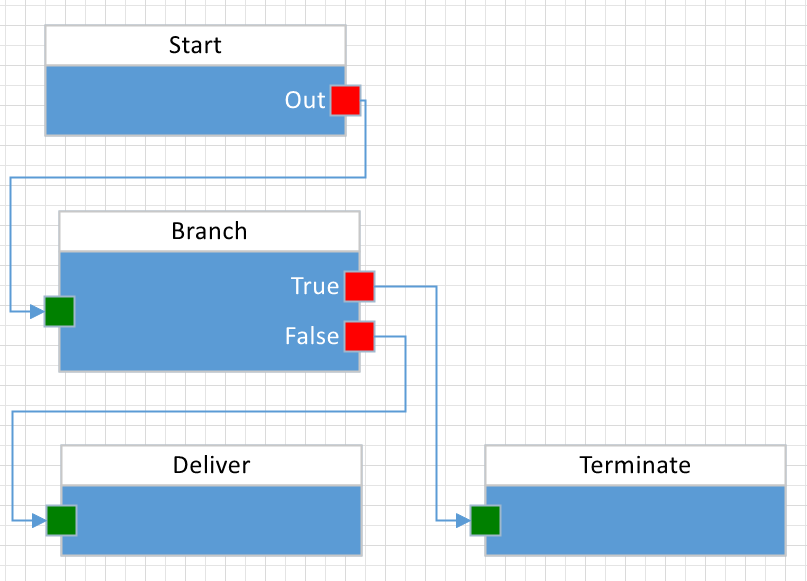
\includegraphics[width=0.7\textwidth]{img/FlowToCodeExample.png}
	\caption[Beispielhaftes Konversationsrouting zur Veranschaulichung der Transformation zu C\#-Syntax]{Beispielhaftes Konversationsrouting zur Veranschaulichung der Transformation zu C\#-Syntax.}
	\label{fig:FlowToCode}
\end{figure}
Am Anfang des Listings steht die Deklaration einer öffentlichen Klasse namens GeneratedConversationBehavior, die von ACDCallRoutingBehavior erbt. Dies ist die Klasse in der die Instruktionen als Membermethoden abgebildet werden. In dieser Klasse wird als nächstes eine private Klasse UserCode definiert. In UserCode sind die vordefinierten Variablen Skill und Language definiert, welche über ihre Getter und Setter auf eine private Instanz des Interfaces IPredefinedVariable zugreifen. Zusätzlich existiert eine Methode mit dem Namen ''BranchNode'' gefolgt von einer einzigartigen Kennnummer. Diese Methode enthält den vom Benutzer spezifizierten Ausdruck der für die Branch-Instruktion ausgeführt werden soll. Dementsprechend wird ein boolescher Wert zurückgeliefert. In diesem Beispiel vergleicht die Branch-Instruktion also die aktuelle Sprache, welche in der vordefinierten Variable Language gespeichert ist, mit dem String ``Deutsch''. 
\newline
Nach der Klasse UserCode folgt die eigentliche Implementierung des Konversationsroutings. Im Konstruktor der Klasse GeneratedConversationBehavior werden Abhängigkeiten zum Rest des System initialisiert: So wird mittels einer Instanz des Interfaces IRoutedAcdCall auf eine API zur Beeinflussung des eingehenden Anrufes zugegriffen. Die beiden Instanzen von IReadOnlyRepository stellen Methoden zur Verfügung, um auf die dem System bekannten Sprachen und Wissensbereiche zuzugreifen. Die drei Interface-Instanzen werden an die Basisklasse ACDCallRoutingBehaviorBase weitergeleitet. Im Konstruktor wird außerdem die private Instanz von UserCode initialisiert, welcher eine Instanz des PredefinedVariables-Interface aus der Basis-Klasse übergeben wird. Die restlichen Methoden der Klassen stellen die Abbildung der Instruktionen des Konversationsroutings dar. Die Start-Instruktion wird auf die Methode ``StartAsync'' abgebildet. Hier wird dem Routing gemäß sofort die Methode der Branch-Instruktion ``BranchNode'' aufgerufen, welche zuerst den vom Benutzerdefinierten Code aus der Klasse UserCode aufruft, und das Ergebnis dessen zur Bedingung in eine If-Abfrage einsetzt. Je nachdem welches Ergebnis zurückgeliefert wird, wird entweder die Methode der Deliver- oder der Terminate-Instruktion aufgerufen. ``TerminateNode'' ruft über die Membervariable Conversation der Basisklasse die API-Methode ``TerminateAsync'' auf, welche den eingehen Anruf beendet. Ähnlich läuft es in ``DeliverNode'' ab: Hier wird der Ruf mittels der API-Methode ``DeliverAsync'' der Ruf an einen Agenten zugestellt. Die dabei übergebene SIP-URI ist ein Parameter der Deliver-Instruktion.
\newline
Wird die Klasse GeneratedConversationBehavior nun von der RoutingEngine instanziert, und in einer Variable vom Typ ACDCallRoutingBehaviorBase gepeichert, kann über die Methode ``StartAsync'' das vom Benutzer gewünschte Konversationsrouting abgespielt werden.

\subsection{Umsetzung}
Das oben beschriebene Konzept zur Abbildung des semantischen Modells auf MSIL-Syntax wird von einer eigenen API realisiert, welche von der Routing Engine benutzt wird. Die grobe Klassenstruktur dieser API ist in Abbildung [UML DIAGRAM] zu sehen. Das Hauptelement ist die Klasse ConversationRoutingBehavior, welche das Interface IBehaviorGenerator implementiert. Dieses Interface stellt die Methode GenerateAssembly zur Verfügung, welche ein semantisches Modell in Form einer Flow-Instanz entgegennimmt und eine MSIL-Assembly zurückliefert. IBehaviorGenerator wird von ConversationRoutingBehaviorGenerator implementiert, welches die Hauptklasse der Transformations-API darstellt. Hier wird der Syntaxbaum des Konversationsroutings erstellt und kompiliert. Zum Erstellen des Syntaxbaums wird die Methode BuildTree des Interfaces ISyntaxTreeBuilder verwendet, welches von der Klasse ConversationRoutingSyntaxTreeBuilder implementiert wird. BuildTree nimmt den Start-Knoten des Konversationsroutings sowie die benutzerdefinierten Variablen und Funktionen entgegen, und liefert einen kompilierbaren Syntaxbaum zurück. Wie dieser Syntaxbaum zusammengesetzt wird, ist in den folgenden Kapiteln erläutert. 

\subsubsection{Programmablauf}
Die Grundidee der Syntax-Zusammensetzung orientiert sich an einem Verfahren, das in [CITATION Voelter S. 272] als ''klassische Modell-Transformierung`` (engl. classical model transformation) bezeichnet wird: Das semantische Modell wird als Graph traversiert, während mit der Roslyn-API anhand des aktuell besuchten Knotens die passende Syntax generiert wird. Die Traversierung beginnt bei dem Start-Knoten des Konversationsroutings und besucht jede Instuktion des Graphen in der Reihenfolge einer Tiefensuche. Pro besuchter Instruktion wird die CLI-Syntax für eine Methode erstellt, welche das Verhalten der Instruktion umsetzt. Dort wo die Syntax die Methode der nachfolgenden Instruktion aufruft, wird rekursiv diese Instruktion besucht und die Syntax für diese nächste Methode erstellt. Dies geht so lange weiter, bis eine Instruktion erreicht wird, die keine ausgehenden Verbindungen hat. An dieser Stelle ist der Rekursionsanker erreicht: Die Syntax für diese Instruktion wird generiert, der Liste der Membermethoden hinzugefügt, und der Aufruf der so generierten Methode an die Vorgänger-Instruktion zurückgeliefert. Diese kann den erhaltenen Aufruf nun in ihre eigene Syntax integrieren und ihren eigenen Aufruf an die eigene Vorgänger-Instruktion zurückliefern. Der Programmfluss kehrt auf diese Weise zurück zur Start-Instruktion, wo der letzte Methodenaufruf in die Methode ``StartAsync'' integriert wird. Zu diesem Zeitpunkt sind alle Methodendeklarationen erstellt und können der Klassendeklaration hinzugefügt werden.
\newline
Da es sich bei einem Konversationsrouting auch um einen zyklischen Graph handeln kann, muss überprüft werden, ob ein Zyklus im aktuellen Routing vorhanden ist, um eine endlose Rekursion zu vermeiden. Daher wird während des rekursiven Ablaufs mit einem Stapelspeicher Protokoll geführt, welche Knoten des Routings schon besucht wurden. Beim Besuchen eines Knotens wird dieser auf den Stapel gelegt, beim Verlassen auf dem Rückweg der Rekursion wird dieser wieder entnommen. Wird ein Knoten besucht, der sich schon auf dem Stapelspeicher befindet, wurde dieser im Zuge eines Zyklus besucht und die Rekursion kann abgebrochen werden. Der zurückzuliefernde Methoden-Aufruf für diesen Knoten wird dann in einem neuen Thread ausgeführt. 
\newline
Die Struktur der Klassen, die den obenstehenden Algorithmus umsetzen, ist in Abbildung [UML DIAGRAM] zu sehen. Die Klasse FlowClassSyntaxBuilder implementiert die Schnittstelle IClassSyntaxBuilder, welche die Methode Build zur Verfügung stellt. Build nimmt eine Referenz auf die StartNode der Klasse Flow entgegen und liefert eine Klassendeklaration in Form einer Roslyn-SyntaxNode zurück. FlowClassSyntaxBuilder implementiert diese Schnittstelle indem es die Syntax für die zu generierende Klasse erstellt. Zum Erstellen der Membermethoden der Klasse wird das Interface IMethodSyntaxBuilder benutzt, welches von der Klasse MethodFlowSyntaxBuilder implementiert wird. IMethodSyntaxBuilder stellt Methoden zur Verfügung, welche Instanzen von Node oder Output entgegen nehmen und eine Methodendeklaration zurückliefern, welche die übergebene Node abbilden soll. MethodFlowSyntaxBuilder implementiert diese Methoden mithilfe des rekursiven Prozesses, der weiter oben erläutert ist. Zu diesem Zweck implementiert die Klasse das Visitor-Pattern in Form des Interfaces IFlowNodeVisitor, in dem Methoden bereit gestellt werden, mit der alle Node-Subtypen sowie Inputs und Outputs besucht werden können. Bei dem Besuch einer Node muss je nach Subtyp bestimmte konkrete CIL-Syntax erstellt werden. Zu diesem Zweck existiert die abstrakte Klasse NodeSyntaxBuilder, von der pro Node-Subtyp eine Klasse erbt, welche die Syntax für den jeweiligen Node-Subtyp in der überschriebenen Build-Methode generiert und an MethodeFlowSyntaxBuilder zurückliefert. Der Ablauf innerhalb der Klasse MethodFlowSyntaxBuilder ist wie folgt: 

\subsubsection{User-Code}
TODO

\subsubsection{Nebenläufigkeit}
TODO

\subsubsection{Benutzerdefinierte Variablen und Funktionen}
TODO

\subsection{Einbindung von generiertem Code}
TODO

\section{Modell-Validierung} 
TODO